\documentclass[a4paper,11pt]{article}

% ----------------- Packages -----------------
\usepackage[utf8]{inputenc}
\usepackage[T1]{fontenc}
\usepackage[english]{babel}
\usepackage{geometry}
\usepackage{amsmath}
\usepackage{graphicx}
\usepackage{tikz}
\usepackage{listings}
\usepackage{xcolor}
\usepackage{hyperref}

\geometry{margin=2.5cm}

% ----------------- Code style -----------------
\lstset{
    language=C++,
    basicstyle=\ttfamily\small,
    keywordstyle=\color{blue},
    commentstyle=\color{gray},
    stringstyle=\color{red!70!black},
    numbers=left,
    numberstyle=\tiny,
    stepnumber=1,
    frame=single,
    breaklines=true,
    showstringspaces=false,
    tabsize=4,
    captionpos=b
}

% ----------------- TikZ styles -----------------
\usetikzlibrary{positioning,arrows.meta,shapes.geometric}
\tikzset{
    stage/.style={
        rectangle, rounded corners,
        draw, minimum width=2.7cm,
        minimum height=1.0cm,
        align=center, font=\small, fill=blue!5
    },
    data/.style={
        trapezium, trapezium left angle=70,
        trapezium right angle=110,
        draw, minimum width=2.6cm,
        minimum height=1.0cm,
        align=center, font=\small, fill=green!5
    }
}

% ----------------- Title -----------------
\title{\textbf{Parallel Longest-Path Detection Using Mapper--Reducer Style}}
\author{Hoang Minh Quan\\ \small Student ID: 23BI14371}
\date{\today}

\begin{document}
\maketitle

\begin{abstract}
This report describes a multithreaded C++ program that finds the longest
paths contained in one or more text files.  The implementation follows a
mapper--reducer style: mapper threads compute the length of each path,
while reducer threads determine the maximum length and collect all paths
that reach this maximum.  The final results are written to an output
file together with their length.
\end{abstract}

\tableofcontents
\newpage

% ----------------- Introduction -----------------
\section{Introduction}

Searching for the longest element in a large collection is a common
pattern in many data-processing tasks.  In this assignment we focus on
\emph{paths} stored as lines in plain text files.  Each line represents
a path encoded as a string (for example, a sequence of node identifiers
or a filesystem path).  Among all available paths, we want to identify
those that have the greatest length measured in characters.

To speed up the computation on multi-core machines, the program uses
several threads organised as mappers and reducers.  The source code is
implemented in standard C++ and uses the STL threading facilities. :contentReference[oaicite:1]{index=1}

% ----------------- Problem description -----------------
\section{Problem Description}

Given:
\begin{itemize}
    \item one or more input text files; each line is treated as a
          candidate path;
    \item an output file name.
\end{itemize}
The program must:
\begin{enumerate}
    \item read all non-empty lines from the input files;
    \item compute the length (in characters) of every path;
    \item determine the maximum path length over the entire dataset;
    \item collect all paths whose length equals this maximum;
    \item write the maximum length and each corresponding path to the
          output file, one per line.
\end{enumerate}

The command-line interface is:
\begin{verbatim}
longestpath <output_file> <input1> [input2 ...]
\end{verbatim}

% ----------------- System overview -----------------
\section{System Overview}

\subsection{High-level Design}

The overall computation is divided into four stages:
\begin{enumerate}
    \item \textbf{Input loading:} all input files are read line by line,
          and non-empty lines are stored in a single vector of strings.
    \item \textbf{Map phase:} the vector of paths is split into
          contiguous chunks.  Each mapper thread receives a chunk and
          produces a list of \texttt{(length, path)} pairs.
    \item \textbf{Reduce phase:} the pairs are partitioned by path
          length and processed by reducer threads.  Each reducer finds
          the local maximum length among its input pairs and remembers
          all paths with that length.
    \item \textbf{Global aggregation:} the maximum length and the
          corresponding set of paths are computed from all reducers, and
          the result is written to the output file.
\end{enumerate}

\subsection{Architecture Illustration}

Figure~\ref{fig:architecture} shows the architecture of the program.
Multiple input files are merged into a single pool of paths, which is
then processed in parallel by mapper and reducer threads.

\begin{figure}[h!]
    \centering
    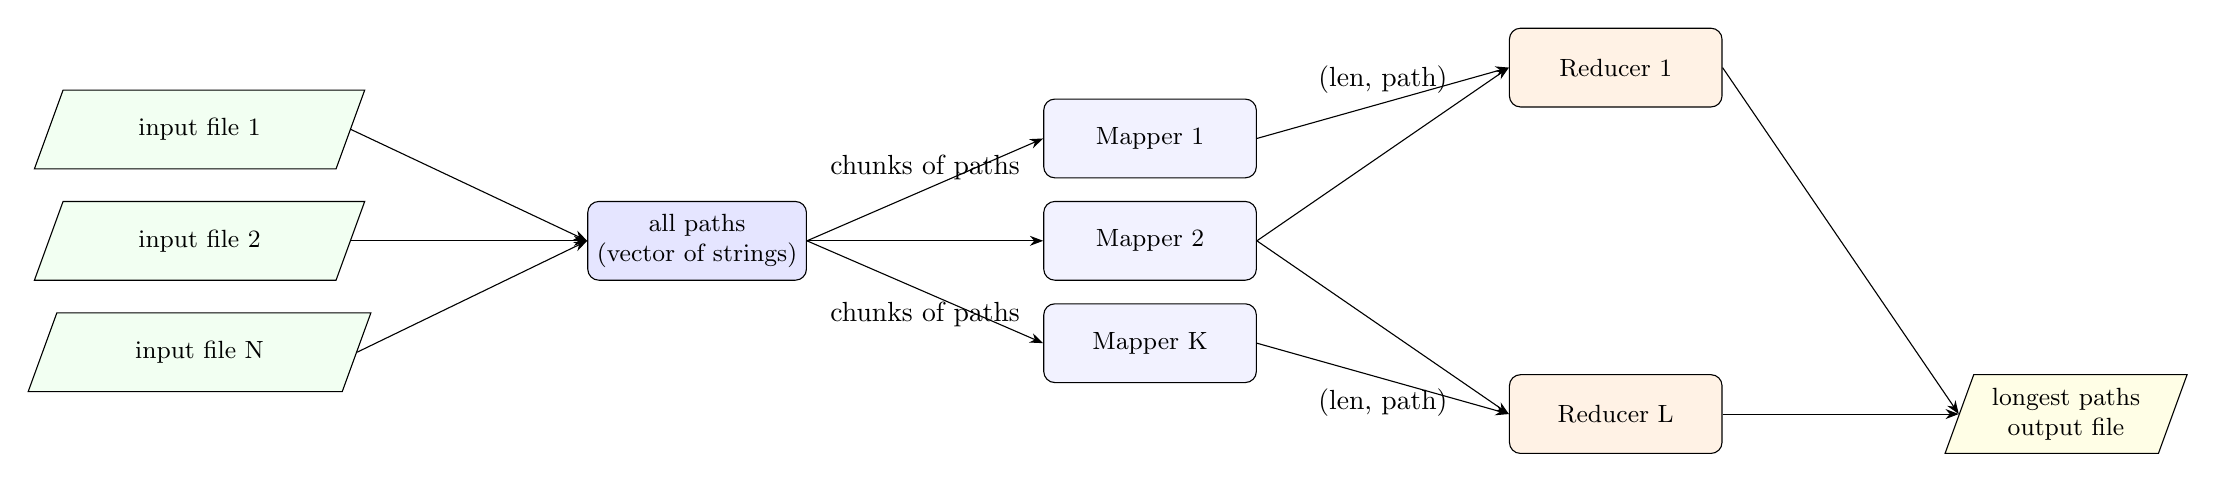
\begin{tikzpicture}[>=Stealth, node distance=1.4cm and 1.6cm]

        % Input files
        \node[data] (in1) {input file 1};
        \node[data, below=0.4cm of in1] (in2) {input file 2};
        \node[data, below=0.4cm of in2] (inN) {input file N};

        % Combined pool
        \node[stage, right=3.0cm of in2, fill=blue!10] (pool)
            {all paths\\(vector of strings)};

        % Mappers
        \node[stage, right=3.0cm of pool, yshift=1.3cm] (m1) {Mapper 1};
        \node[stage, right=3.0cm of pool] (m2) {Mapper 2};
        \node[stage, right=3.0cm of pool, yshift=-1.3cm] (m3) {Mapper K};

        % Reducers
        \node[stage, right=3.2cm of m1, fill=orange!10, yshift=0.9cm] (r1)
            {Reducer 1};
        \node[stage, right=3.2cm of m3, fill=orange!10, yshift=-0.9cm] (r2)
            {Reducer L};

        % Output
        \node[data, right=3.0cm of r2, fill=yellow!10] (out)
            {longest paths\\output file};

        % Arrows from input files to pool
        \draw[->] (in1.east) -- (pool.west);
        \draw[->] (in2.east) -- (pool.west);
        \draw[->] (inN.east) -- (pool.west);

        % Arrows to mappers
        \draw[->] (pool.east) -- node[above]{chunks of paths} (m1.west);
        \draw[->] (pool.east) -- (m2.west);
        \draw[->] (pool.east) -- node[below]{chunks of paths} (m3.west);

        % Arrows to reducers
        \draw[->] (m1.east) -- node[above]{(len, path)} (r1.west);
        \draw[->] (m2.east) -- (r1.west);
        \draw[->] (m2.east) -- (r2.west);
        \draw[->] (m3.east) -- node[below]{(len, path)} (r2.west);

        % Arrows to output
        \draw[->] (r1.east) -- (out.west);
        \draw[->] (r2.east) -- (out.west);

    \end{tikzpicture}
    \caption{Mapper--reducer style architecture for longest-path detection.}
    \label{fig:architecture}
\end{figure}

% ----------------- Implementation -----------------
\section{Implementation Details}

\subsection{Data Structures}

Two main structures are used in the program:
\begin{itemize}
    \item a \texttt{std::vector<std::string>} storing all paths read
          from the input files;
    \item a \texttt{ReducerResult} structure for each reducer, holding
          the local maximum length and the list of paths achieving this
          length:
\begin{verbatim}
struct ReducerResult {
    int max_len = 0;
    std::vector<std::string> paths;
};
\end{verbatim}
\end{itemize}

Mapper threads output vectors of \texttt{(length, path)} pairs, which
are then redistributed among reducers based on the hash of the length.

\subsection{Mapper Threads}

The function \texttt{mapper\_worker} receives the global vector of paths
and a range \texttt{[begin, end)} indicating which paths it should
process.  For each path, it computes its length (in characters) and
appends a pair \texttt{(length, path)} to the output vector.

The main thread divides the total number of paths into approximately
equal chunks.  When the number of paths is smaller than the requested
number of mappers, the program automatically reduces the mapper count to
avoid idle threads.

\subsection{Reducer Threads}

Reducer threads take vectors of \texttt{(length, path)} pairs as input.
Each reducer scans its pairs and keeps track of:
\begin{itemize}
    \item the largest length it has seen so far, and
    \item the list of paths that have exactly that length.
\end{itemize}

When a longer path appears, the reducer updates its local maximum and
resets the list of stored paths to contain only the new longest path.
When a path ties the current maximum, it is appended to the list.

Hash partitioning on the integer length is used to distribute pairs to
reducers:
\begin{equation}
    \text{reducer\_id} = \text{hash}(\text{len}) \bmod \text{num\_reducers}.
\end{equation}

\subsection{Global Aggregation and Output}

After all reducers have finished, the main thread scans the
\texttt{ReducerResult} structures to compute a global maximum length and
a combined list of paths:
\begin{itemize}
    \item if a reducer reports a larger maximum, its paths replace the
          current global list;
    \item if a reducer reports the same maximum, its paths are appended
          to the global list.
\end{itemize}

Finally, each path whose length equals the global maximum is written to
the output file in the form:
\begin{verbatim}
<max_length> <path>
\end{verbatim}

% ----------------- Source Code -----------------
\section{Source Code Listing}

For completeness, Listing~\ref{lst:code} contains the full code of the
program.

\begin{lstlisting}[caption={C++ implementation of parallel longest-path detection},
                   label={lst:code}]
#include <algorithm>
#include <fstream>
#include <iostream>
#include <string>
#include <thread>
#include <unordered_map>
#include <utility>
#include <vector>

struct ReducerResult {
    int max_len = 0;
    std::vector<std::string> paths;
};

void mapper_worker(const std::vector<std::string>& all_paths,
                   size_t begin, size_t end,
                   std::vector<std::pair<int, std::string>>& out_pairs) {
    for (size_t i = begin; i < end; ++i) {
        const std::string& p = all_paths[i];
        int len = static_cast<int>(p.size());
        out_pairs.emplace_back(len, p);
    }
}

void reducer_worker(const std::vector<std::pair<int, std::string>>& in_pairs,
                    ReducerResult& out_result) {
    int local_max = 0;
    std::vector<std::string> local_paths;
    for (const auto& kv : in_pairs) {
        int len = kv.first;
        const std::string& path = kv.second;
        if (len > local_max) {
            local_max = len;
            local_paths.clear();
            local_paths.push_back(path);
        } else if (len == local_max) {
            local_paths.push_back(path);
        }
    }
    out_result.max_len = local_max;
    out_result.paths = std::move(local_paths);
}

int main(int argc, char** argv) {
    if (argc < 3) {
        std::cerr << "Usage: " << argv[0]
                  << " <output_file> <input1> [input2 ...] \n";
        return 1;
    }

    std::string output_file = argv[1];
    std::vector<std::string> input_files;
    for (int i = 2; i < argc; ++i) {
        input_files.push_back(argv[i]);
    }

    std::vector<std::string> all_paths;
    for (const auto& fname : input_files) {
        std::ifstream in(fname);
        if (!in.is_open()) {
            std::cerr << "Cannot open input file: " << fname << "\n";
            return 1;
        }
        std::string line;
        while (std::getline(in, line)) {
            if (!line.empty())
                all_paths.push_back(line);
        }
        in.close();
    }

    if (all_paths.empty()) {
        std::cerr << "No paths found in input files.\n";
        return 1;
    }

    int num_mappers = 4;
    int num_reducers = 2;
    if (static_cast<int>(all_paths.size()) < num_mappers) {
        num_mappers = static_cast<int>(all_paths.size());
    }
    if (num_reducers > num_mappers) {
        num_reducers = num_mappers;
    }

    std::vector<std::thread> mapper_threads;
    std::vector<std::vector<std::pair<int, std::string>>> mapper_outputs(num_mappers);

    size_t total = all_paths.size();
    size_t base_chunk = total / num_mappers;
    size_t extra = total % num_mappers;
    size_t start = 0;

    for (int i = 0; i < num_mappers; ++i) {
        size_t chunk = base_chunk + (i < static_cast<int>(extra) ? 1 : 0);
        size_t end = start + chunk;
        mapper_threads.emplace_back(mapper_worker,
                                    std::cref(all_paths),
                                    start, end,
                                    std::ref(mapper_outputs[i]));
        start = end;
    }

    for (auto& t : mapper_threads) t.join();

    std::vector<std::vector<std::pair<int, std::string>>> reducer_inputs(num_reducers);
    for (const auto& m_out : mapper_outputs) {
        for (const auto& kv : m_out) {
            int len = kv.first;
            size_t h = std::hash<int>{}(len);
            int rid = static_cast<int>(h % num_reducers);
            reducer_inputs[rid].push_back(kv);
        }
    }

    std::vector<std::thread> reducer_threads;
    std::vector<ReducerResult> reducer_results(num_reducers);

    for (int r = 0; r < num_reducers; ++r) {
        reducer_threads.emplace_back(reducer_worker,
                                     std::cref(reducer_inputs[r]),
                                     std::ref(reducer_results[r]));
    }

    for (auto& t : reducer_threads) t.join();

    int global_max = 0;
    std::vector<std::string> longest_paths;

    for (const auto& res : reducer_results) {
        if (res.max_len > global_max) {
            global_max = res.max_len;
            longest_paths = res.paths;
        } else if (res.max_len == global_max) {
            longest_paths.insert(longest_paths.end(),
                                 res.paths.begin(), res.paths.end());
        }
    }

    if (global_max == 0) {
        std::cerr << "Could not compute longest path length.\n";
        return 1;
    }

    std::ofstream out(output_file);
    if (!out.is_open()) {
        std::cerr << "Cannot open output file: " << output_file << "\n";
        return 1;
    }

    for (const auto& p : longest_paths) {
        if (static_cast<int>(p.size()) == global_max)
            out << global_max << " " << p << "\n";
    }
    out.close();

    std::cout << "Longest path length: " << global_max
              << ", number of paths: " << longest_paths.size() << "\n";
    std::cout << "Results written to: " << output_file << "\n";

    return 0;
}
\end{lstlisting}

% ----------------- Usage Example -----------------
\section{Usage Example}

After compiling the program with a C++17-capable compiler, for example:
\begin{verbatim}
g++ -std=c++17 -pthread longestpath.cpp -o longestpath
\end{verbatim}
it can be executed as:
\begin{verbatim}
./longestpath results.txt paths1.txt paths2.txt
\end{verbatim}
The file \texttt{results.txt} will then contain the maximum path length
followed by each path that achieves this length.

% ----------------- Conclusion -----------------
\section{Conclusion}

The longest-path program illustrates how a mapper--reducer style design
can be used in a multithreaded C++ application.  By splitting the input
set of paths among mapper threads and combining partial maxima with
reducers, the solution is able to exploit several CPU cores while
keeping the code relatively simple.  The same pattern could be reused
for other aggregation tasks, such as finding the shortest path, the most
frequent pattern, or computing summary statistics over large datasets.

\end{document}
